% !TeX program = lualatex

\documentclass[12pt,a4paper]{book}
\usepackage[utf8]{inputenc}
\usepackage[T1]{fontenc}

\usepackage[version=4]{mhchem}
\usepackage{stmaryrd}
\usepackage{multirow}
\usepackage[export]{adjustbox}

\usepackage[galician]{babel}
\usepackage{amsmath}
\usepackage{amsthm}
\usepackage{amsfonts}
\usepackage{amssymb}
\usepackage{titlesec}
\usepackage{graphicx}
\usepackage{mathtools}
%\usepackage{mathabx}
\author{\huge \textsf{Grado en Matemáticas}}
\title{\Huge \textbf{\textsc{Álgebra Lineal y Multilineal}}}
\usepackage{array}
\usepackage{float}
\setlength{\parindent}{0pt}
\usepackage[a4paper]{geometry}
\geometry{top=2.5cm, bottom=2.5cm, left=3.00cm, right=3.00cm}
\usepackage{fancyhdr}
\pagestyle{headings}
\usepackage{color}
\usepackage{cancel}
\usepackage{ulem}
\usepackage{tcolorbox}
\usepackage{multirow}
\usepackage{tikz}
\usetikzlibrary{babel, arrows.meta, arrows, datavisualization, patterns}
\usepackage{multicol}
\usepackage{stackrel}
\usepackage{pdfpages}
\usepackage{pgfplots}
\pgfplotsset{compat=1.15}
\renewcommand{\labelitemi}{\textbullet}
\newcommand{\li}{\ell}
\newcommand{\grad}{\text{grad }}
\newcommand{\rad}{\text{rad}}
\newcommand{\mcm}{\text{mcm }}
\newcommand{\mcd}{\text{mcd }}
\newcommand{\eva}{\text{ev}_{\alpha}}
\newcommand\ndots{\stackrel{\mathclap{\normalfont\mbox{\scriptsize($n$)}}}{\cdots}}
\newcommand\sdots{\stackrel{\mathclap{\normalfont\mbox{\scriptsize($s$)}}}{\cdots}}
\newcommand\rddots{\stackrel{\mathclap{\normalfont\mbox{\scriptsize($r$)}}}{\ddots}}
\newcommand\pddots{\stackrel{\mathclap{\normalfont\mbox{\scriptsize($p$)}}}{\ddots}}
\newcommand\qddots{\stackrel{\mathclap{\normalfont\mbox{\scriptsize($q$)}}}{\ddots}}
\newcommand\nrddots{\stackrel{\mathclap{\normalfont\mbox{\scriptsize($n-r$)}}}{\ddots}}
\newcommand{\dsum}{\displaystyle\sum}

\theoremstyle{definition}

\newcommand\dint{\displaystyle\int}

\newcommand{\boundellipse}[3]% center, xdim, ydim
{(#1) ellipse (#2 and #3)
}


\newtheorem{ejemplo}{\textbf{Ejemplo}}
\newtheorem{ejer}{\textbf{Ejercicio}} 
\newtheorem{defi}{\textbf{Definición}} 
\newtheorem{theorem}{\textbf{Teorema}} 
\newtheorem{lema}{\textbf{Lema}} 
\newtheorem{corol}{\textbf{Corolario}} 
\newtheorem{prop}{\textbf{Proposición}}
\newtheorem{nota}{\textbf{\textit{Nota}}}
\newtheorem{nt}{\textit{Notación}}
\newtheorem{obvi}{\textbf{Observación}}
\newtheorem{ctr}{\textit{Contraejemplo}}

\usepackage{fancyhdr}
\pagestyle{fancy}

\fancyhead[RE]{\rightmark}     
\fancyhead[LO]{\leftmark}     
\fancyhead[RO]{\thepage}     
\fancyhead[LE]{\thepage}
\fancyfoot[LE]{\logo Gallaecia}
\fancyfoot[RE]{Memoria}
\fancyfoot[LO]{\logo Gallaecia}
\fancyfoot[RO]{Memoria}
\fancyfoot[CE]{\textcolor{white}{}}
\fancyfoot[CO]{\textcolor{white}{}}

\newtheoremstyle{break}
{\topsep}{\topsep}%
{\itshape}{}%
{\bfseries}{}%
{\newline}{}%
\theoremstyle{break}
\newtheorem*{intr}{\textit{Interpretación geométrica}}

\renewcommand\qedsymbol{$\blacksquare$}

\usepackage{hyperref}
\hypersetup{
	colorlinks,
	citecolor=black,
	filecolor=black,
	linkcolor=black,
	urlcolor=black
}

\usepackage{listings}
\lstset{ frame=Ltb,
	framerule=0pt,
	aboveskip=0.5cm,
	framextopmargin=3pt,
	framexbottommargin=3pt,
	framexleftmargin=0cm,
	framesep=0pt,
	rulesep=.4pt,
	backgroundcolor=\color{gray97},
	rulesepcolor=\color{black},
	%
	stringstyle=\ttfamily,
	showstringspaces = false,
	basicstyle=\small\ttfamily,
	commentstyle=\color{gray45},
	keywordstyle=\bfseries,
	%
	numbers=left,
	numbersep=10pt,
	numberstyle=\tiny,
	numberfirstline = false,
	breaklines=true,
}

% minimizar fragmentado de listados
\lstnewenvironment{listing}[1][]
{\lstset{#1}\pagebreak[0]}{\pagebreak[0]}

\lstdefinestyle{consola}
{basicstyle=\footnotesize\bf\ttfamily,
	backgroundcolor=\color{gray85},
}

\lstdefinestyle{sql}
{language=sql,
}

\decimalpoint

\newcommand{\inlinecode}[2]{\colorbox{gray85}{\lstinline[language=#1,style=consola]$#2$}}

\usepackage{tocloft}

\usepackage{wrapfig}

\usepackage{tikz-cd}

\usepackage{xcolor, colortbl}
\definecolor{blueice}{rgb}{.85, .96, .94}
\definecolor{lightcopper}{RGB}{255, 245, 234}


\newenvironment{contraejemplo}
{\begin{figure}[H] \centering \begin{tabular} {p{.085\textwidth} | p{.875\textwidth}}
			\begin{wrapfigure}{l}{\linewidth}
				\includegraphics[width=\linewidth,angle=10]{alerta.pdf}
				\vspace{-10pt}
			\end{wrapfigure} & \begin{ctr} }
			{\end{ctr}
\end{tabular} \end{figure}}

\newenvironment{interpretacion}[1]
{\begin{figure} [H] \centering \begin{tabular} {| p{.5\textwidth} | p{.44\textwidth} |}
			\hline
			\begin{theorem}
				#1
			\end{theorem}  &
			\textcolor{white}{.}
			
			\textbf{\textit{Interpretación geométrica.}}}
		{\textcolor{white}{.}\\
			\hline
\end{tabular} \end{figure}}

\newenvironment{interpretacion-corol}[1]
{\begin{figure} [H] \centering \begin{tabular} {| p{.5\textwidth} | p{.44\textwidth} |}
			\hline
			\begin{corol}
				#1
			\end{corol}  &
			\textcolor{white}{.}
			
			\textbf{\textit{Interpretación geométrica.}}}
		{\textcolor{white}{.}\\
			\hline
\end{tabular} \end{figure}}


\usepackage{unicode-math}
\setmathfont{TeX Gyre Schola Math}
%\usepackage[sfdefault]{firasans}
\usepackage{amsmath}
\usepackage{amssymb}\setmainfont{Times New Roman}

%\setmathfont{STIX Two Math}
\setmathfont{LatinModern-Math.otf}[range=\sum]
\setmathfont{Cambria Math}[range=\in]

% IMPORTANTE: Corregir error del SETMINUS

\usepackage{pgfplots}
\pgfplotsset{compat=1.15}
\usepackage{mathrsfs}
\usetikzlibrary{arrows}
\usepackage{changepage}


\setmathfont{LatinModern-Math.otf}[range=\mitalpha]
\setmathfont{Cambria Math}[range=\int]

\newfontfamily{\logo}{CourierNew Bold}[]

\addto\captionsspanish{
	\renewcommand{\chaptername}{Sección}
}

\usepackage[indent=30pt]{parskip}

\usepackage[hang, small,labelfont=bf,up,textfont=it,up]{caption} % Custom captions under/above floats in tables or figures

\definecolor{gris}{RGB}{224, 224, 224}

\setlength{\arrayrulewidth}{0.4mm}
\renewcommand{\baselinestretch}{1.15}

\addto\captionsgalician{
	\renewcommand{\chaptername}{Sección}
}

\definecolor{gray97}{gray}{.97}
\definecolor{gray85}{gray}{.85}
\definecolor{gray45}{gray}{.45}

\usepackage{tablefootnote}


\begin{document}
	\begin{titlepage}
		\begin{adjustwidth}{-1.5cm}{}
			\begin{tabular}{p{2.4cm}p{15cm}}
				
\includegraphics[width=3.4cm]{logo_ux.jpg}
				\begin{center}
					\rule[2cm]{0.8mm}{19.5cm}%vertical
					\hspace{1pt}
					\rule[2cm]{0.4mm}{19.5cm}%vertical
				\end{center}
				&
				\vspace{-2.5cm}
				\begin{center}
					\rule[1mm]{15cm}{0.4mm}%horizontal
					\vspace{0.1pt}
					\rule[3mm]{15cm}{0.8mm}%horizontal
					\\
					\LARGE{\bf{Universidade de Santiago de Compostela}}\\
					\vspace*{0.3cm}
					\large{\bf{Escola Técnica Superior de Enxeñaría}}
					
					\vspace{3\baselineskip}
					{\Huge{{\logo GALLAECIA}}}\\
					\vspace*{0.2cm}
					{\Large \textbf{Implementación de la aplicación}}
					
					\vspace*{0.9cm}
					\Large{\bf MEMORIA}
					
					\vspace*{0.9cm}
					{\large \bf{Presentada por:}}
					
					\vspace*{0.5cm}
					{\LARGE \bf{Carlos Cao López}}\\
					\vspace*{0.2cm}
					{\LARGE \bf{Adrián Eitor Morrazo}}\\
					\vspace*{0.2cm}
					{\LARGE \bf{Yago Falgueras Casarejos}}\\
					\vspace*{0.2cm}
					{\LARGE \bf{Ignacio Garbayo Fernández}}\\
					\vspace*{0.2cm}
					{\LARGE \bf{Pedro Vidal Villalba}}
					
					\vspace*{0.7cm}
					{\large \bf{Miembros del Grupo 3A}}
					
					\vspace*{1.1cm}
					{\large \bf{Para la materia:}}\\
					\vspace*{0.3cm}
					\huge{\bf Bases de Datos II}
					
					\vspace*{1cm}
					
					{\large \bf{Santiago de Compostela}}\\
					\vspace*{-0.4cm}
					{\large \bf{2023}}
				\end{center}
			\end{tabular}
		\end{adjustwidth}
	\end{titlepage}
	\newpage
	\textcolor{white}{text}
	\thispagestyle{empty}
	\newpage
	\tableofcontents
	
	\newpage
	\listoffigures
	\listoftables
	
	\chapter{Motivación}
	
	O obxectivo deste proxecto é crear unha conexión a unha base de datos e manexar diferentes transaccións e vistas de forma didáctica sobre ela. Para isto, non se comeza desde cero, senón que se parte do proxecto dun compañeiros doutro ano realizado en Bases de Datos I. Os autores deste son Marta Ceán Romero, Paula Dobato Mouriz, Laura Salgueiro Sánchez e Artur Vázquez Rego. Sobre o seu traballo, vanse xuntar as aportacións individuais do anexo ao modelo base, e cambiar algúns aspectos co obxectivo de melloralo onde sexa posible. 
	
	Polo tanto, mostrarase unha versión nova da semántica, modelo conceptual, dicionario de datos e modelo lóxico na parte de deseño. Con respecto á implementación, crearase unha conexión á base de datos desde un programa escrito en Java, que permitirá a diferentes usuarios acceder a ela e consultar información sobre certas tablas ás que teñan permiso de acceso. Esta é a parte principal do proxecto, na que se aprenderá tanto sobre o funcionamento interno das bases de datos e os posibles problemas ocasionados por ter varios usuarios operando nela simultáneamente, como sobre a programación dunha conexión entre Java e a base de datos, e a creación dunha interfaz gráfica sinxela que permita visualizar e modificar algúns elementos da base de datos.
	
	Para poder mostrar esta última parte, adxuntaranse os códigos de creación da base de datos, da inserción de algúns datos aleatorios e operarase sobre eles mediantes algunhas transaccións. 
	
	Debido á complexidade do proceso, creouse un diagrama de Gantt cunha breve planificación na que se recollen as partes máis relevantes do proxecto xunto coa súa data estimada de comezo e duración aproximada. 
	
	\begin{figure} [H] \centering
		\caption{Diagrama de Gantt}
		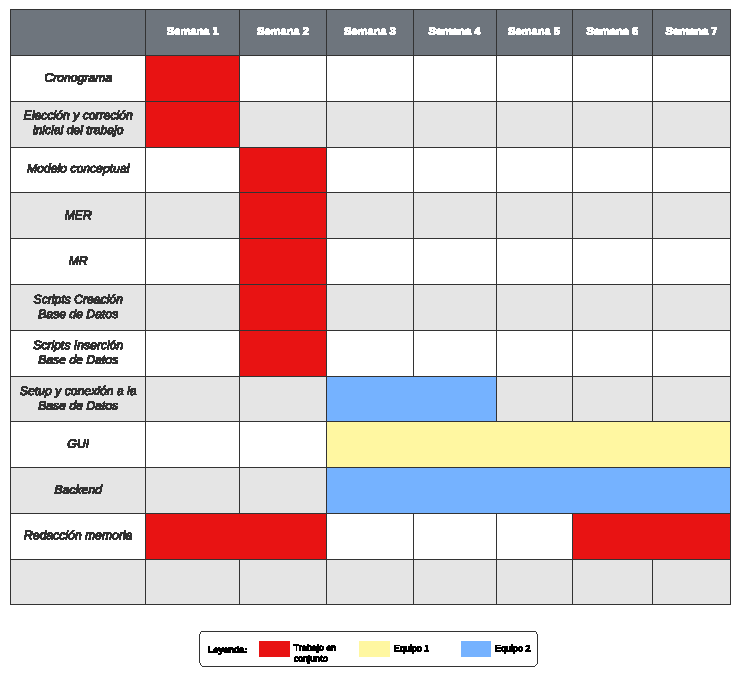
\includegraphics[width=\textwidth]{Diagrama de Gantt.pdf}
	\end{figure}
	
	
	\chapter{Análise Semántica}
	Con motivo da próxima apertura do Parque Temático {\logo Gallaecia}, decidiuse crear unha base de datos para xestionar toda a información relativa á mesma.
	
	\section{Descrición}
	O Parque Temático {\logo Gallaecia}, n'As Illas Cíes, desexa manter unha base de datos con información sobre as súas diferentes atraccións e empresas asociadas. Para iso, precisa almacenar unha lista das atraccións ofertadas, así coma datos sobre cada un dos visitantes, empregados, hoteles e restaurantes vinculados, entre outros. Ademais, é preciso recoller todos os valores relacionados cos espectáculos.
	
	De cada unha das feiras quérese almacenar o seu nome (que debe ser distinto para cada unha), ubicación, aforo, prezo de mantemento, altura mínima requerida e unha descrición de outros aspectos de interese.
	
	Das persoas que deciden pasar por {\logo Gallaecia} é preciso coñecer o seu DNI, nome e nacionalidade. Así mesmo, deséxase gardar tanto o seu teléfono de contacto como a súa data de nacemento e altura, esta última imprescindible para poder gozar dos entretementos. Cabe destacar que se necesita calcular a idade do visitante. Ademais, de cada un precísase saber as atraccións, espectáculos e restaurantes aos que foi. Cómpre destacar que só se quere gardar os días nos que asistiu ás diferentes actividades, non se acudiu varias veces nun mesmo día.
	
	Todas as atraccións deben ser controladas por empregados do parque, dos que se garda o DNI, nome, teléfono, dirección (con rúa, número, código postal e localidade), data de nacemento e idade. Relacionados directamente co parque, outros datos de interese recollidos serían o seu salario e a súa formación completa na actividade que desempeña, así coma o tempo que leva traballando con {\logo Gallaecia}.
	
	Outro factor a ter en conta é que os empregados se dedican, entre outras cousas, a actuar en espectáculos e a manter en correcto estado todas as atraccións do parque. En canto aos hoteis e restaurantes, basta saber o seu nome, ubicación, aforo e horario, incluíndo neste último a súa hora de apertura e peche.
	
	{\logo Gallaecia} tamén garda información sobre os diversos espectáculos nos que actúan os empregados. Destes necesitaríase tanto o seu nome coma a súa temática, ubicación e horario. Para coñecer exactamente que ofrece cada espectáculo, deberíase incluir tamén unha breve descrición.
	
	Por outro lado, o parque contará con diferentes zonas onde se sitúan as distintas atraccións e restaurantes, e onde se representan os espectáculos. Interésanos gardar o seu nome (único para cada zona) e a súa extensión en metros cadrados.
	
	Como engadido, o parque de atraccións {\logo Gallaecia} desexa incluír na súa actual base de datos información sobre as súas diferentes formas de ambientar con música. Para iso, necesita almacenar unha lista da música, así como datos sobre cada un dos DJ que
	se encargan da súa reprodución e dos sistemas de audio distribuídos polas
	diversas zonas.
	
	De cada un dos sistemas de son quérese almacenar un número identificador, a súa función, unha breve descrición sobre os mesmos e a súa localización no
	parque.
	
	En canto á música, é preciso coñecer un código identificativo de cada canción
	ou obra musical; así como o seu nome, clasificación e popularidade. Por diferentes motivos relacionados cos DJ, deséxase gardar, ademais, tanto o artista como o
	álbum dos diferentes temas que se reproducirán.
	Como xa se mencionou, todos os sistemas de audio deben ser controlados por empregados
	do parque. Destes, como xa se especificou na semántica da base de datos
	inicial, gárdase o DNI, nome, teléfono, dirección...
	
	Ademais, cabe destacar que un traballador pode exercer o seu labor ou ben na
	hostelería, ou ben como axudante do parque ou como DJ. Os DJ encárganse de controlar
	os sistemas de audio previamente mencionados.
	
	A maiores do comentado anteriormente, o Parque Temático {\logo Gallaecia} precisa
	manter certa orde nas atraccións para facilitar o manexo dos datos. Para isto necesita categorizalas segundo distintos tipos: atraccións nas que só poden montar adultos a partir de determinados anos; e feiras familiares, nas que poden montar todos os visitantes pero das
	que gardaremos tamén unha idade mínima recomendada a partir da cal o disfrute
	será maior.
	
	Por último, hai que sumar agora os medios de transporte que
	van permitir acceder ao parque. Destes interesa saber datos coma o prezo, a
	capacidade, o tempo que lle leva chegar, o tipo (mariño ou aéreo) e por último o
	nome, que será único.
	Ademais, gardarase que medio emprega cada visitante para chegar, só podendo
	usar un para tal fin.
	
	\section{Datos}
	\begin{itemize}
		\item \textbf{Atraccións}: nome, aforo, altura mínima para montar, custo do mantemento, ubicación, descrición.
		
		\item \textbf{Atraccións só para adultos}: idade mínima requerida para montar na atracción.
		
		\item \textbf{Atraccións familiares}: idade recomendada para montar na atracción.
		
		\item \textbf{Visitantes}: DNI, nome, nacionalidade, teléfono, data de nacemento, altura, idade.
		
		\item \textbf{Hostalaría}: nome do establecemento, ubicación, aforo, hora de inicio, hora de fin.
		
		\item \textbf{Espectáculos}: nome, hora de inicio, hora de finalización, temática, descrición, ubicación.
		
		\item \textbf{Empregados}: DNI, nome, dirección na que habitan (rúa, número, código postal, localidade), salario, teléfono, data na que comezaron a traballar no parque, data de nacemento, formación, idade, tempo que levan traballando no parque, se son hostaleiros ou se son traballadores de parque ou DJ.
		
		\item \textbf{Zonas}: nome, extensión, coordenadas da ubicación.
		
		\item \textbf{Música}: código de cada canción, nome da canción, clasificación, popularidade, artista, álbum.
		
		\item \textbf{Sistemas de audio}: número identificador de cada sistema, función, breve
		descrición, localización.
		
		\item \textbf{Medios}: nome, capacidade, tempo en chegar (velocidade), prezo e o tipo (mariño ou aéreo).
	\end{itemize}
	
	
	
	\section{Transaccións}
	\begin{itemize}
		\item \textbf{T1}: eliminar un restaurante e asignar eses hostaleiros a outro.
		
		\item \textbf{T2}: ao traballador que leva menos tempo traballando no parque e só traballa nunha atracción queremos asignarlle un espectáculo e subirlle o salario.
		
		\item \textbf{T3}: xubilamos a un hostaleiro e reducimos o aforo do restaurante asociado.
		
		\item \textbf{T4}: consultar o nome e a altura dos visitantes que foron a máis de 3 atraccións ordenados de forma descendente segundo o número de atraccións.
		
		\item \textbf{T5}: consultar nome, aforo, altura mínima e descrición da atracción máis visitada.
		
		\item \textbf{T6}: consultar o número de persoas totales que visitaron o parque cunha idade comprendida entre 17 e 29 anos.
		
		\item \textbf{T7}: consultar os traballadores que levan traballando máis tempo que a media dos empregados do seu tipo.
		
		\item \textbf{T8}: consultar nome, salario e formación dos traballadores do restaurante máís visitado.
		
		\item \textbf{T9}: consultar cal dos espectáculos da tarde (despois das 16h) tivo máis afluencia entre 2015 e 2018.
		
		\item \textbf{T10}: consultar o espectáculo que conta con máis traballadores.
		
		\item \textbf{T11}: consultar que anos hai perdas e cales ganancias, baixo a fórmula
		$$\text{no. visitantes}\times \text{prezoEntradaMantemento}.$$
		
		\item \textbf{T12}: Consultar o nome, a idade e a nacionalidade dos visitantes que coincidiron con algún dos traballadores que máis cobra e ademais foron ao restaurante onde a suma dos salarios dos hostaleiros é a maior.
		
		\item \textbf{T13}: Consultar cal é a estación na que hai máis afluencia nas atraccións.
		
	\end{itemize}
	
	
	\chapter{Modelo Conceptual}
	Neste apartado presentarase a información referida ao modelo conceptual, no cal optamos por facer unha única vista.
	
	Partindo da Semántica atopamos as seguintes entidades: as atraccións que compoñen o parque (\textbf{Atraccións}), os seus visitantes (\textbf{Visitantes}), os diferentes establecementos hostaleiros (\textbf{Hostalaría}), as actuacións e entretementos (\textbf{Espectáculos}) e os diferentes traballadores (\textbf{Empregados}). Para reflectir mellor a relación destes últimos cos outros entes, optamos por separalos nunha xerarquía. Por unha banda os que traballan na hostalaría (\textbf{Hostaleiros}) e por outra o resto de persoal encargado das atraccións e espectáculos (\textbf{TraballadoresParque}).
	
	Entre as devanditas entidades, reflectindo a Semántica, temos as consecuentes relacións: os visitantes poden (\textbf{Xantar}) nos establecementos hostaleiros, (\textbf{Ir}) ás atraccións ou (\textbf{Asistir}) aos espectáculos; todas elas relacións $N:N$ das que nos interesa gardar a Data. Cada traballador do parque está encargado de (\textbf{Manter}) unha atracción ou (\textbf{Actuar}) nunha función. Por último, os hostaleiros van (\textbf{Traballar}) nun dos locais de comida.
	
	Coas aportacións do anexo aparecen as seguintes novas entidades: a música que ambienta o
	parque (\textbf{Música}), os sistemas de son que a reproducen (\textbf{Sistemas de audio}),
	e os traballadores específicos (\textbf{DJ}), que engádense á xerarquía de (\textbf{Empregados}).
	
	Entre estas novas entidades e reflectindo a Semántica, hai a seguinte relación: os DJ poden (\textbf{Controlar}) os sistemas de audio. Ademais, cada sistema
	de audio do parque encárgase de (\textbf{Reproducir}) unha serie de obras musicais determinadas. Interesa gardar a data na que se reproduce unha determinada
	canción nun sistema de audio.
	
	Para reflectir os tipos de atraccións construímos unha xerarquía formada por: \textbf{SóAdultos} e
	\textbf{Familiares}. Esta é total (pois só existen esas categorías e todas as atraccións se
	identifican con ao menos unha) e disxunta (unha atracción non pode ser á vez de varios
	tipos).
	
	Por outro lado, a nove entidade (\textbf{Zonas}) permite ubicar ás atraccións mediante a relación (\textbf{SituarseAtracción}), aos establecementos de hostalaría con (\textbf{SituarseHostalaría}), aos espectáculos do parque con (\textbf{SituarseEspectáculo}) e aos sistemas de audio con (\textbf{Situarse Audio}).
	
	Finalmente, ao modelo conceptual anterior engádese a seguinte entidade: os medios de transporte para chegar á illa (\textbf{Medios}). Entre estes e os (\textbf{Visitantes}) aparece a relación (\textbf{Viaxar}).
	
	
	\newpage
	
	\section{Modelo Entidade-Relación}
	
	\begin{figure} [H] \centering
		\caption{Diagrama Entidade-Relación}
		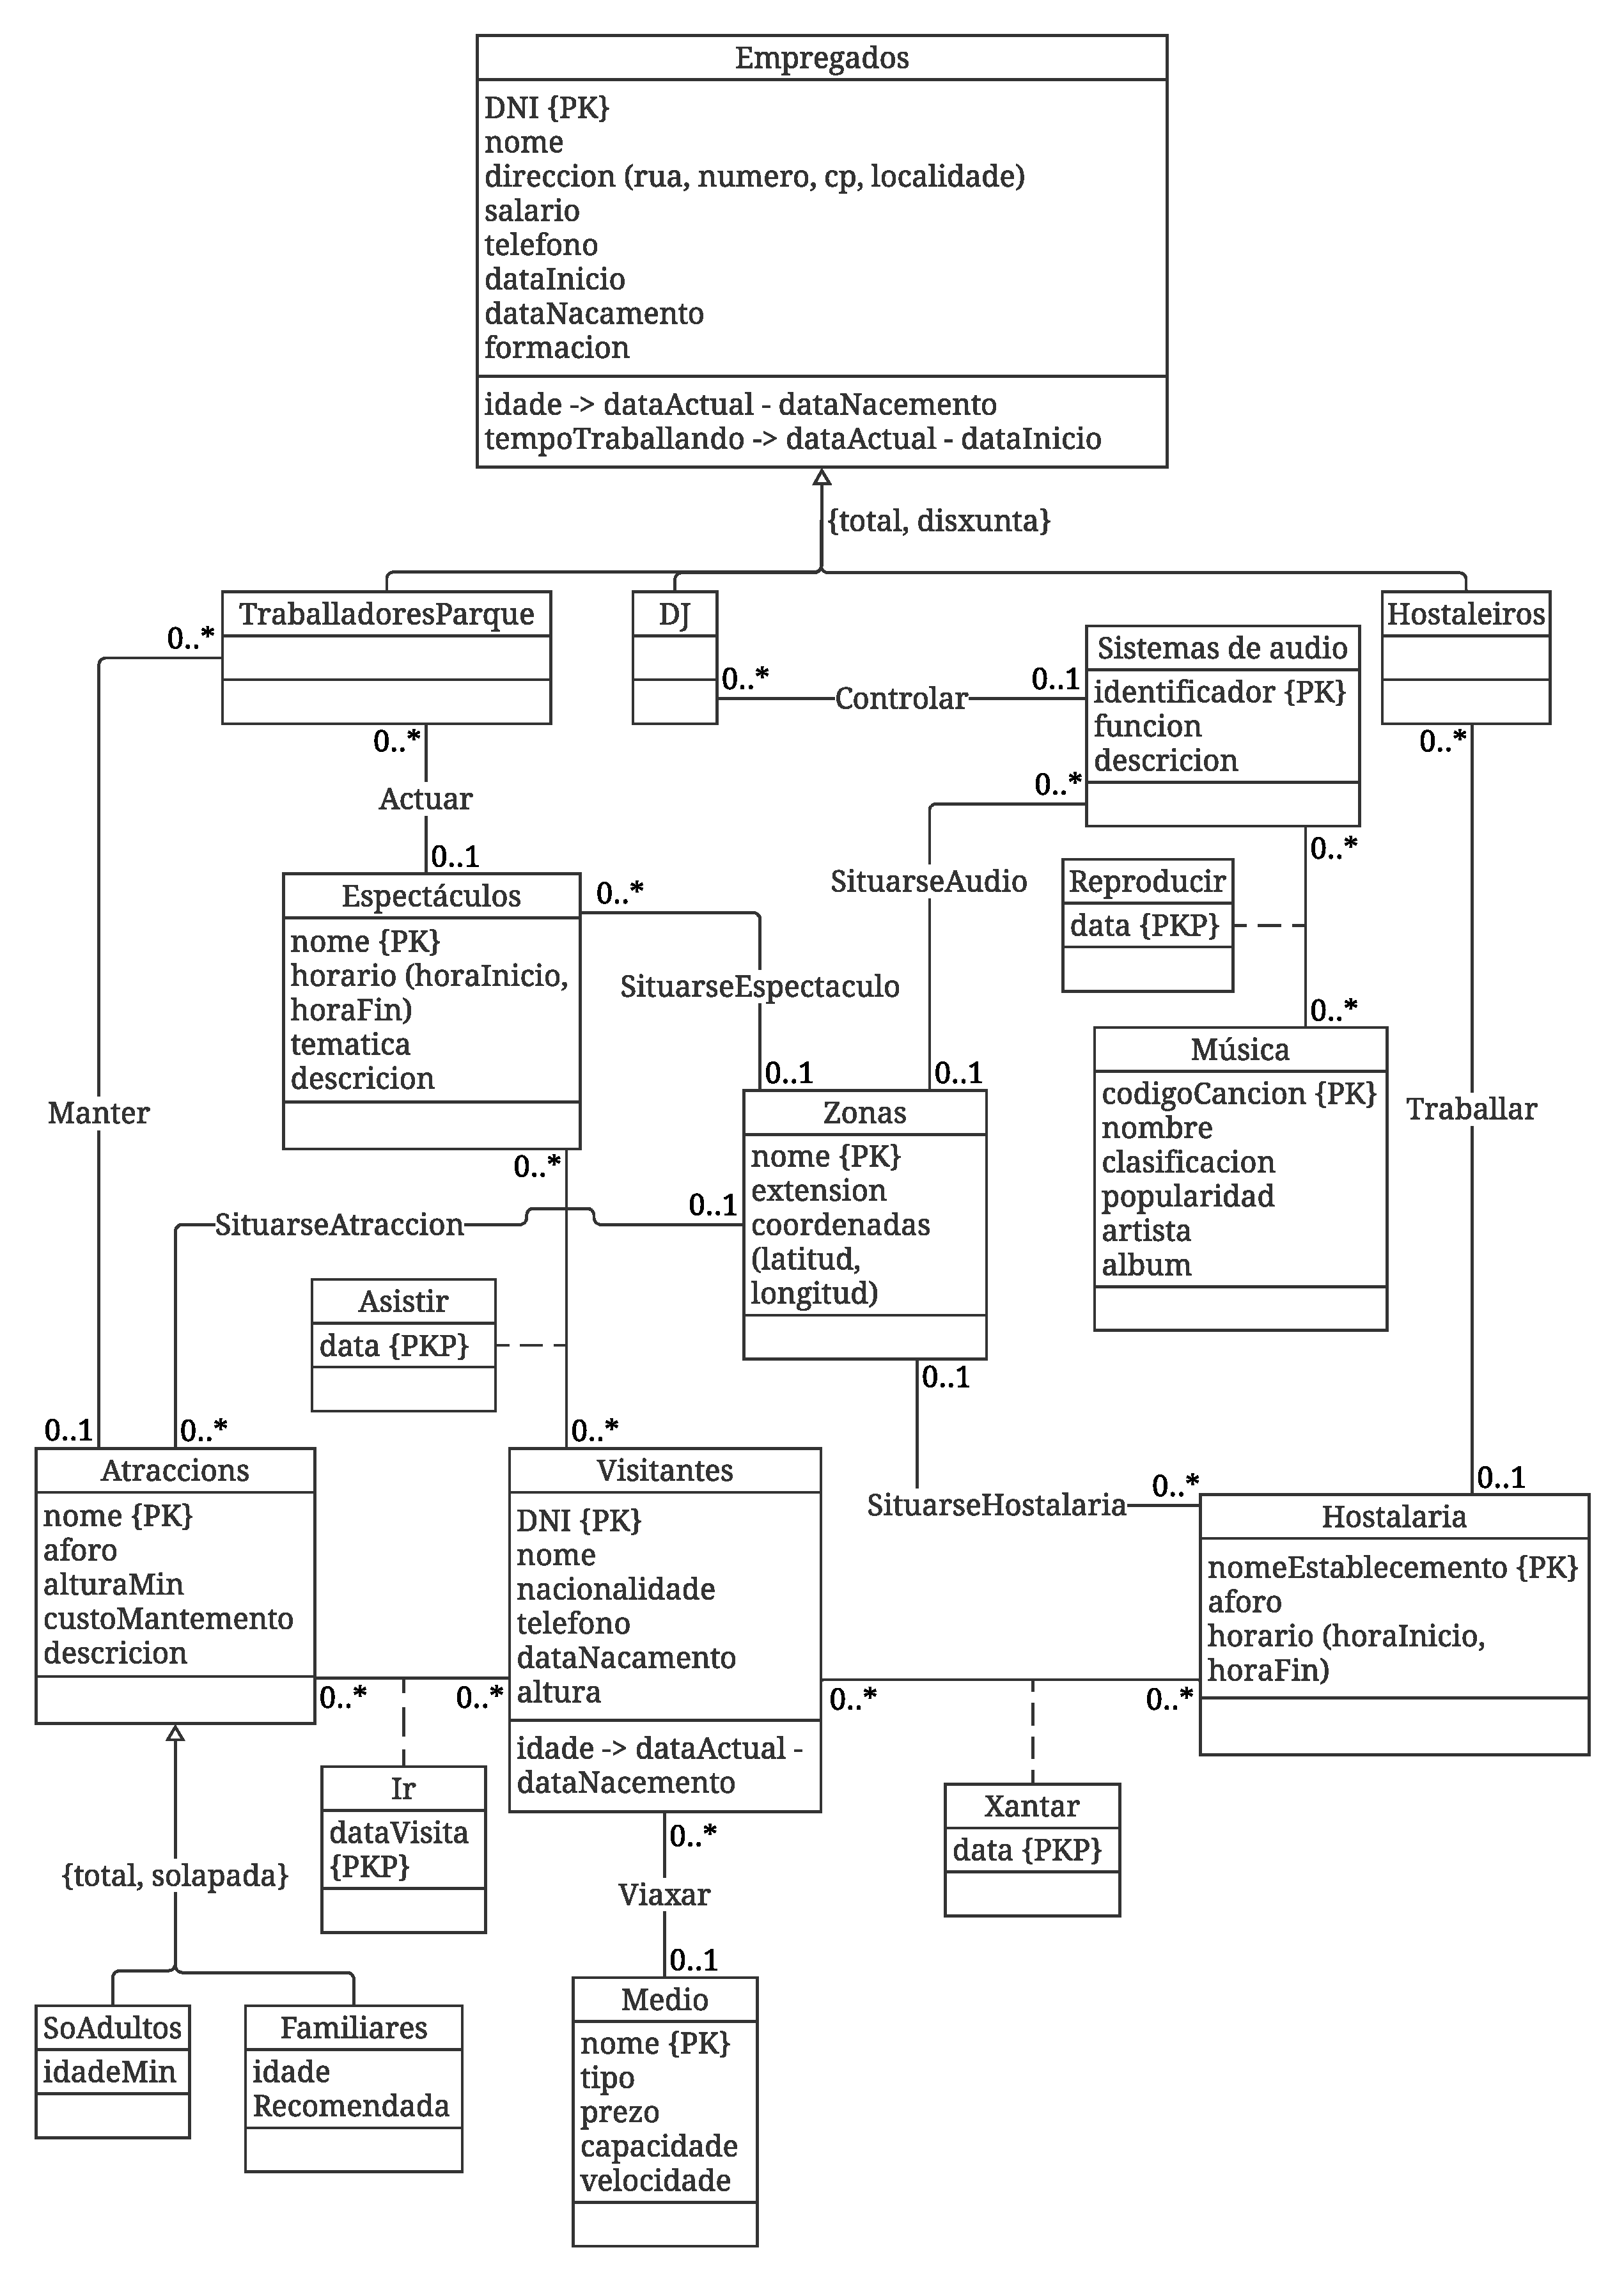
\includegraphics[width=\textwidth]{MER inicial.pdf}
	\end{figure}
	\newpage
	
	\section{Dicionario de Datos}
	
	Terase en conta que \textbf{N} ven a abreviar «admite nulos». Ademais, dado que non hai atributos multivalorados e non se asinan valores por defecto, prescíndese destas dúas columnas.
	
	\begin{table} [H] \centering
		\caption{Glosario de entidades\\}
		\begin{tabular}{|m{2.5cm}|m{5.5cm}|m{5.5cm}|}
			\hline \rowcolor{gris}
			\multicolumn{1}{|c|}{Entidades} & \multicolumn{1}{c|}{Descrición} & \multicolumn{1}{c|}{Número de instancias} \\
			\hline
			Atraccións & Datos das atraccións que conforman o parque & Número de atraccións existentes \\
			\hline
			Visitantes & Datos das persoas que visitan o parque & Número de persoas que visitan o parque \\
			\hline
			Hostalaría & Datos dos establecemento hostaleiros do parque & Número de establecementos \\
			\hline
			Espectáculos & Datos dos espectáculos que organiza o parque & Número de espectáculos que realiza o parque \\
			\hline
			Empregados & Datos empregados que traballan para o parque & Número de empregados que traballan no parque \\
			\hline
			Traballadores do Parque & Datos dos empregados que traballan no mantemento do parque (ou espectáculos) & Número de traballadores do parque \\
			\hline
			Hostaleiros & Traballadores da hostalaría do parque & Número de empregados hostaleiros  \\
			\hline
			Zonas & Datos das zonas que  compoñen o parque & Número de zonas existentes\\
			\hline
			Sistemas de audio &  Datos dos sistemas de son que compoñen o parque & Número de aparatos existentes\\
			\hline
			Música &  Datos da música que soa no parque & Número de cancións\\
			\hline
			DJ &  Datos dos DJ que pinchan no parque & Número de DJ existentes\\
			\hline
			SóAdultos & Datos de atraccións para adultos existentes & Número de atraccións para adultos existentes \\
			\hline
			Familiares & Datos de atraccións familiares existentes & Número de atraccións  familiares existentes \\
			\hline
			Medios & Datos dos medios de transporte para chegar & Número de medios  dispoñibles \\
			\hline
		\end{tabular}
	\end{table}
	
	\newpage
	
	\begin{table} [H] \centering
		\caption{Glosario de relacións}
		\begin{tabular}{|m{2.3cm}|c|m{2.05cm}|c|m{2.4cm}|}
			\hline \rowcolor{gris}
			\multicolumn{1}{|c|}{Entidade} & \multicolumn{1}{c|}{Multiplicidade} & \multicolumn{1}{c|}{Relación} & \multicolumn{1}{c|}{Multiplicidade} & \multicolumn{1}{c|}{Entidade} \\
			\hline
			Atraccións & $*$ & Ir & $*$ & Visitantes \\
			\hline
			Atraccións & $0$..$1$ & Manter & $*$ & Traballadores Parque \\
			\hline
			Visitantes & $*$ & Xantar & $*$ & Hostalaría \\
			\hline
			Visitantes & $*$ & Asistir & $*$ & Espectáculos \\
			\hline
			Espectáculos & $0$..$1$ & Actuar & $*$ & Traballadores Parque \\
			\hline
			Hostalaría & $0$..$1$ & Traballar & $*$ & Hostaleiros \\
			\hline
			Zonas & $0$..$1$ & Situarse Atracción & $*$ & Atracccións\\
			\hline
			Zonas & $0$..$1$ & Situarse Hostalaría & $*$ & Hostalaría\\
			\hline
			Zonas & $0$..$1$ & Situarse \textcolor{white}{aa} Espectáculo & $*$ & Espectáculos\\
			\hline
			Zonas & $0$..$1$ & Situarse Audio & $*$ & Sistemas de audio\\
			\hline
			DJ & $*$ & Controlar & $0$..$1$ & Sistemas de audio\\
			\hline
			Sistemas de audio & $*$ & Reproducir & $*$ & Música\\
			\hline
			Medios & 1 & Viaxar & $*$& Visitantes\\
			\hline
		\end{tabular}
	\end{table}
	
	
	\newpage
	
	\begin{table} [H] \centering
		\caption{Glosario de atributos}
		\begin{tabular}{|c|m{3cm}|m{4cm}|m{2cm}|m{0.7cm}|}
			\hline \rowcolor{gris}
			\multicolumn{1}{|m{2.5cm}|}{Entidade ou relación} & \multicolumn{1}{c|}{Atributos} & \multicolumn{1}{c|}{Descrición} & \multicolumn{1}{m{2cm}|}{Tipos de datos} & \multicolumn{1}{c|}{$\mathbf{N}$} \\
			\hline
			\multirow{5}{*}{\textbf{Atraccións}} & \texttt{nome} (PK) &  Nome único para cada atracción do parque &  carácter \textcolor{white}{aa} variable 30 & non \\
			\cline{2-5}
			& \texttt{aforo} & Número máximo de persoas que soporta a atracción & enteiro & non \\
			\cline{2-5}
			& \texttt{alturaMin} & Altura mínima necesaria para poder subir á atracción & enteiro & non \\
			\cline{2-5}
			& \texttt{custo Mantemento} & Custo medio de manter en boa situación á atracción & real & si \\
			\cline{2-5}
			& \texttt{descrición} & Características principais da atracción &  carácter \textcolor{white}{aa} variable  500 & si \\
			\hline
			\multirow{7}{*}{\textbf{Visitantes}} & \texttt{DNI} (PK) & DNI do visitante & carácter 9 & non \\
			\cline{2-5}
			& \texttt{nome} & Nome e apelidos do visitante & carácter \textcolor{white}{aa} variable 60 & non \\
			\cline{2-5}
			& \texttt{nacionalidade} & País do visitante & carácter \textcolor{white}{aa} variable 30 & si \\
			\cline{2-5}
			& \texttt{teléfono} & Número de teléfono do visitante & carácter 9 & si \\
			\cline{2-5}
			& \texttt{data Nacemento} & Data de nacemento do visitante en formato ddmmaaa & data & si \\
			\cline{2-5}
			& \texttt{altura} & Altura do visitante en $\mathrm{cm}$ & enteiro & non \\
			\cline{2-5}
			& \texttt{idade}\tablefootnote{\texttt{idade} é un atributo calculado: \texttt{idade} $=$ \texttt{dataActual} $-$ \texttt{dataNacemento}} & Idade do visitante & enteiro & si \\
			\hline
			\multirow{3}{*}{\textbf{Zonas}} & \texttt{nome} (PK) & Nome único para cada zona do parque &  carácter \textcolor{white}{aa} variable 30 & non \\
			\cline{2-5}
			& \texttt{extension} & Superficie en m$^2$ que ocupa cada zona & real & si \\
			\cline{2-5}
			& \texttt{coordenadas} & Latitude e lonxitude da ubicación & punto & si \\
			\hline
		\end{tabular}
	\end{table}
	
	\newpage
	
	
	\begin{table} [H] \centering
		\begin{tabular}{|c|m{3cm}|m{4cm}|m{2cm}|m{0.7cm}|}
			\hline \rowcolor{gris}
			\multicolumn{1}{|m{2.5cm}|}{Entidade ou relación} & \multicolumn{1}{c|}{Atributos} & \multicolumn{1}{c|}{Descrición} & \multicolumn{1}{m{2cm}|}{Tipos de datos} & \multicolumn{1}{c|}{$\mathbf{N}$} \\
			\hline
			\multirow{4}{*}{\textbf{Hostalaría}} & \texttt{nome Establecemento} (PK) & Nome único para cada establecemento &  carácter \textcolor{white}{aa} variable 30 & non \\
			\cline{2-5}
			& \texttt{aforo} & Capacidade máxima do establecemento & enteiro & non \\
			\cline{2-5}
			& \texttt{horaInicio} & Hora á que abre o establecemento & tempo & si \\
			\cline{2-5}
			& \texttt{horaFin} & Hora á que pecha o establecemento & tempo & si \\
			\hline
			\multirow{5}{*}{\textbf{Espectáculos}} & \texttt{nome} (PK) & Nome único para cada espectáculo que se realice &  carácter \textcolor{white}{aa} variable 30 & non \\
			\cline{2-5}
			& \texttt{horaInicio} & Hora á que comeza o espectáculo & tempo & si \\
			\cline{2-5}
			& \texttt{horaFin} & Hora á que remata o espectáculo & tempo & si \\
			\cline{2-5}
			& \texttt{temática} & Temática do espectáculo &  carácter \textcolor{white}{aa} variable 15 & si \\
			\cline{2-5}
			& \texttt{descrición} & Explicación breve sobre a actuación &  carácter \textcolor{white}{aa} variable 200 & si \\
			\hline
			\multirow{5}{*}{\textbf{Medios}} & \texttt{nome} (PK) & nome único para cada medio de transporte &  carácter \textcolor{white}{aa} variable 30 & non\\
			\cline{2-5}
			& \texttt{tipo} & tipo de transporte (mariño ou aéreo) &  carácter \textcolor{white}{aa} variable 30 & non\\
			\cline{2-5}
			&\texttt{prezo} & custo dunha viaxe & real & non\\
			\cline{2-5}
			&\texttt{capacidade} & número máximo de persoas que pode levar & enteiro & non\\
			\cline{2-5}
			&\texttt{velocidade} & tempo en chegar ata a illa en minutos & real & non\\
			\hline
		\end{tabular}
	\end{table}
	
	\newpage
	
	\begin{table} [H] \centering
		\begin{tabular}{|c|m{3cm}|m{4cm}|m{2cm}|m{0.7cm}|}
			\hline \rowcolor{gris}
			\multicolumn{1}{|m{2.5cm}|}{Entidade ou relación} & \multicolumn{1}{c|}{Atributos} & \multicolumn{1}{c|}{Descrición} & \multicolumn{1}{m{2cm}|}{Tipos de datos} & \multicolumn{1}{c|}{$\mathbf{N}$} \\
			\hline
			\multirow{13}{*}{\textbf{Empregados}} & \texttt{DNI} (PK) & DNI do traballador & carácter 9 & non \\
			\cline{2-5}
			& \texttt{nome} & Nome do traballador & carácter \textcolor{white}{aa} variable 60 & non \\
			\cline{2-5}
			& \texttt{rúa} & Rúa onde vive o traballador & carácter \textcolor{white}{aa} variable 40 & si \\
			\cline{2-5}
			& \texttt{número} & Número do edificio onde vive o traballador & enteiro & si \\
			\cline{2-5}
			& \texttt{cp} & Código postal da dirección do traballador & enteiro & si \\
			\cline{2-5}
			& \texttt{localidade} & Localidade da residencia do traballador &  carácter \textcolor{white}{aa} variable 30 & si \\
			\cline{2-5}
			& \texttt{salario} & Cantidade mensual que cobra o traballador & real & non \\
			\cline{2-5}
			& \texttt{teléfono} & Teléfono móbil do traballador & carácter 9 & si \\
			\cline{2-5}
			& \texttt{dataInicio} & Data de inicio do traballador no parque & data & non \\
			\cline{2-5}
			& \texttt{data Nacemento} & Data de nacemento do traballador & data & si \\
			\cline{2-5}
			& \texttt{formación} & Currículo profesional do traballador &  carácter \textcolor{white}{aa} variable 100 & non \\
			\cline{2-5}
			& \texttt{idade}\tablefootnote{\texttt{idade} é un atributo calculado: \texttt{idade} $=$ \texttt{dataActual} $-$ \texttt{dataNacemento}} & Idade do traballador & enteiro & si \\
			\cline{2-5}
			& \texttt{tempo Traballado}\tablefootnote{\texttt{tempoTraballado} é un atributo calculado: \texttt{tempoTraballado} $=$ \texttt{dataActual} $-$ \texttt{dataInicio}}  &  Tempo que o traballador leva traballando no parque & enteiro & si \\
			\hline
			\textbf{Ir} & \texttt{dataVisita} (PKP) & Data na que un visitante vai ao parque & data & non \\
			\hline
			\textbf{Xantar} & \texttt{data} (PKP) & Día no que o visitante xanta nun establecemento do parque & data & non \\
			\hline
			\textbf{Asistir} & \texttt{data}(PKP) & Día no que o visitante acode a un espectáculo do parque & data & non \\
			\hline
		\end{tabular}
	\end{table}
	
	\newpage
	
	\begin{table} [H] \centering
		\begin{tabular}{|c|m{3cm}|m{4cm}|m{2cm}|m{0.7cm}|}
			\hline \rowcolor{gris}
			\multicolumn{1}{|m{2.5cm}|}{Entidade ou relación} & \multicolumn{1}{c|}{Atributos} & \multicolumn{1}{c|}{Descrición} & \multicolumn{1}{m{2cm}|}{Tipos de datos} & \multicolumn{1}{c|}{$\mathbf{N}$} \\
			\hline
			\textbf{Reproducir} & \texttt{data Reproducción} (PKP) & Data na que se reproduce unha canción nun sistema de audio determinado & data & non\\
			\hline
			\multirow{3}{*}{$\begin{array}{c}
					\text{\textbf{Sistemas de}}\\\text{\textbf{audio}}
			\end{array}$} & \texttt{identificador} (PK) & código único para cada sistema do parque & carácter 5 & non\\
			\cline{2-5}
			&\texttt{función} & tipo de aparato de audio &  carácter \textcolor{white}{aa} variable 20 & non\\
			\cline{2-5}
			& \texttt{descripción} & características principais do aparato de son &  carácter \textcolor{white}{aa} variable 150 & sí\\
			\cline{2-5}
			\hline
			\multirow{6}{*}{\textbf{Música}} & \texttt{codigo Canción} & código identificativo & carácter 9 & non\\
			\cline{2-5}
			& \texttt{nome} & título da canción &  carácter \textcolor{white}{aa} variable 30 & non\\
			\cline{2-5}
			&\texttt{clasificación} & xénero da canción &  carácter \textcolor{white}{aa} variable 30 & non\\
			\cline{2-5}
			& \texttt{popularidade} & valoración do $1$ ao $100$ & enteiro & non\\
			\cline{2-5}
			& \texttt{artista} & nome do autor da obra &  carácter \textcolor{white}{aa} variable 30 & non\\
			\cline{2-5}
			& \texttt{álbum} & nome do álbum da canción &  carácter \textcolor{white}{aa} variable 30 & non\\
			\hline
			\textbf{SóAdultos} & \texttt{idadeMin} & idade mínima requerida para o acceso & enteiro & si\\
			\hline
			\textbf{Familiares} & \texttt{idade Recomendada } & idade recomendada para o acceso & enteiro & si\\
			\hline 
			
		\end{tabular}
	\end{table}
	
	\chapter{Modelo Lóxico}
	O modelo Entidade-Relación e o Relacional son representacións diferentes, tanto conceptual coma loxicamente, dunha base de datos. Coma os Xestores de bases adoitan empregar o modelo Relacional, neste apartado transformaremos o modelo entidade-relación nun modelo relacional aplicando unha serie de regras.
	
	En primeiro lugar, cada unha das entidades do MER pasan a ser unha relación. Para o caso das entidades febles, inclúen tamén a clave primaria parcial da entidade da que dependen.
	
	En canto ás xerarquías (neste caso, total e disxunta) cada entidade convírtese, ao igual ca sempre, nunha relación. Así mesmo, as subclases pasarán a ter a mesma clave que as superclases. Isto afecta aos Empregados. Na xerarquía de Atraccións non se segue o estándar: crearase unha relación para a superclase porque esta ten varias relación con outras entidades. 
	
	Por outra banda, é preciso converter as relacións $1:N$ e $N:N$. Nas binarias $1:N$, inclúese unha copia da clave primaria do lado $1$ na táboa do lado $N$. Ademais, introdúcense os atributos da relación na táboa do lado $N$. Nas relacións $N:N$ procédese de forma diferente: cada unha transfórmase nunha relación nova, coa combinación das claves primarias das entidades que une coma clave primaria.
	
	Para os atributos compostos hai que descompoñelos en atributos atómicos.
	
	Finalmente e relacionado coas \textbf{claves externas}, é preciso analizar as políticas de integridade referencial e os casos relacionados con estas. Interésanos gardar a información actual ao parque, non a relativa aos datos pasados. Polo tanto, en xeral, a actualización será en \texttt{cascade}, para manter os datos coherentes. A eliminación, por temas de protección de datos será, salvo algunha ocasión, tamén en \texttt{cascade}. Porén, cando se trate das atraccións, espectáculos ou establecementos dos traballadores, será \texttt{set null}. Isto é porque temporalmente poden estar sen ningún asignado.
	
	\newpage
	\section{Modelo Relacional}
	O Modelo Relacional resultante da análise anterior é o seguinte.
	
	\begin{lstlisting} [language=sql,style=sql,tabsize=5, escapechar={|},
		keywordstyle=\color{blue}\ttfamily,
		stringstyle=\color{red}\ttfamily]
 |\color{red}ZONAS| (nome, extensión, coordenadaX, coordenadaY)
	|\color{blue}Clave primaria|: nome
	|\color{violet}Forma normal|: BC
	
 |\color{red}ATRACCIÓNS| (nome, aforo, alturaMin, custoMantemento, zona, descrición)
 	|\color{blue}Clave primaria|: nome
 	|\color{violet}Forma normal|: BC
 	|\color{teal}Clave externa|: zona |\color{teal}REFERENCIA| |\color{red}Zonas|(nome)
 		Borrado: set null, Actualización: cascade
		
 |\color{red}ATRACCIÓNSSÓADULTOS| (nome, idadeMin)
	|\color{blue}Clave primaria|: nome
	|\color{violet}Forma normal|: BC
	|\color{teal}Clave externa|: nome |\color{teal}REFERENCIA| |\color{red}Atraccións|(nome)
		Borrado: set null, Actualización: cascade
		
 |\color{red}ATRACCIÓNSFAMILIARES| (nome, idadeRecomendada)
	|\color{blue}Clave primaria|: nome
	|\color{violet}Forma normal|: BC
	|\color{teal}Clave externa|: nome |\color{teal}REFERENCIA| |\color{red}Atraccións|(nome)
		Borrado: set null, Actualización: cascade
		
 |\color{red}MEDIOS| (nomeMedio, tipo, prezo, capacidade, velocidade)
	|\color{blue}Clave primaria|: nome
	|\color{violet}Forma Normal|: BC
		
 |\color{red}VISITANTES| (DNI, nome, nacionalidade, teléfono, dataNacemento, altura, idade, medioTransporte) 
	|\color{blue}Clave primaria|: DNI
	|\color{violet}Forma normal|: BC
	|\color{orange}Atributo derivado|: idade --> dataActual - dataNacemento
	|\color{teal}Clave externa|: medioTransporte |\color{teal}REFERENCIA| |\color{red}Medios|(nomeMedio)
		Borrado: set null, Actualización: cascade
		
		
		
		
		
		
 |\color{red}IR| (dataVisita, visitante, atracción)
	|\color{blue}Clave primaria|: dataVisita, visitante, atracción
	|\color{violet}Forma normal|: BC
	|\color{teal}Clave externa|: visitante |\color{teal}REFERENCIA| |\color{red}Visitantes|(DNI)
		Borrado: cascade, Actualización: cascade
	|\color{teal}Clave externa|: atracción |\color{teal}REFERENCIA| |\color{red}Atraccións|(nome)
		Borrado: cascade, Actualización: cascade
		
 |\color{red}HOSTALARÍA| (nomeEstablecemento, zona, aforo, horaInicio, horaFin)
	|\color{blue}Clave primaria|: nomeEstablecemento
	|\color{violet}Forma Normal|: BC
	|\color{teal}Clave externa|: zona |\color{teal}REFERENCIA| |\color{red}Zonas|(nome)
		Borrado: set null, Actualización: cascade
		
 |\color{red}XANTAR| (data, visitante, establecemento)
	|\color{blue}Clave primaria|: data, visitante, establecemento
	|\color{violet}Forma normal|: BC
	|\color{teal}Clave externa|: visitante |\color{teal}REFERENCIA| |\color{red}Visitantes|(DNI)
		Borrado: cascade, Actualización: cascade
	|\color{teal}Clave externa|: establecemento |\color{teal}REFERENCIA| |\color{red}Hostalaría|(nome Establecemento)
		Borrado: cascade, Actualización: cascade
		
 |\color{red}ESPECTÁCULOS| (nome, horaInicio, horaFin, temática, descrición, zona)
	|\color{blue}Clave primaria|: nome
	|\color{violet}Forma normal|: BC
	|\color{teal}Clave externa|: zona |\color{teal}REFERENCIA| |\color{red}Zonas|(nome)
		Borrado: set null, Actualización: cascada
		
 |\color{red}ASISTIR| (data, visitante, espectáculo)
	|\color{blue}Clave primaria|: data, visitante, espectáculo
	|\color{violet}Forma normal|: BC
	|\color{teal}Clave externa|: visitante |\color{teal}REFERENCIA| |\color{red}Visitantes|(DNI)
		Borrado: cascade, Actualización: cascade
	|\color{teal}Clave externa|: espectáculo |\color{teal}REFERENCIA| |\color{red}Espectáculos|(nome)
		Borrado: cascade, Actualización: cascade
		
		
		
		
		
		
		
		
 |\color{red}TRABALLADORESPARQUE| (DNI, nome, rúa, número, cp, localidade, salario, teléfono, dataInicio, dataNacemento, formación, idade, tempoTraballando nomeAtracción, nomeEspectáculo)
	|\color{blue}Clave primaria|: DNI
	|\color{violet}Forma Normal|: BC
	|\color{teal}Clave externa|: nomeAtracción |\color{teal}REFERENCIA| |\color{red}Atraccións|(nome)
		Borrado: set null, Actualización: cascade
	|\color{teal}Clave externa|: nomeEspectáculo |\color{teal}REFERENCIA| |\color{red}Espectáculos|(nome)
		Borrado: set null, Actualización: cascade
	|\color{orange}Atributo Derivado|: idade --> dataActual - dataNacemento
	|\color{orange}At. Derivado|: tempoTraballando --> dataActual - dataInicio
		
 |\color{red}HOSTALEIROS| (DNI, nome, rúa, número, cp, localidade, salario, teléfono, dataInicio, dataNacemento, formación, idade, nomeEstablecemento)
	|\color{blue}Clave primaria|: DNI
	|\color{violet}Forma Normal|: BC
	|\color{teal}Clave externa|: nomeEstablecemento |\color{teal}REFERENCIA| |\color{red}Hostalaría|(nomeEstablecemento)
		Borrado: set null, Actualización: cascade
	|\color{orange}Atributo Derivado|: idade --> dataActual - dataNacemento
	|\color{orange}At. Derivado|: tempoTraballando --> dataActual - dataInicio
		
 |\color{red}MÚSICA| (codigoCancion, nome, clasificación, popularidade, artista, álbum)
	|\color{blue}Clave primaria|: codigoCancion
	|\color{violet}Forma normal|: BC
		
 |\color{red}SISTEMASDEAUDIO| (identificador, función, descrición, zona)
	|\color{blue}Clave primaria|: identificador
	|\color{violet}Forma normal|: BC
	|\color{teal}Clave externa|: zona |\color{teal}REFERENCIA| |\color{red}Zonas|(nome)
		Borrado: set null, Actualización: cascade
		
 |\color{red}DJ| (DNI, nome, calle, número, cp, localidade, salario, teléfono, dataInicio, dataNacemento, formación, idade, tempoTraballando, identificadorSistema)
	|\color{blue}Clave primaria|: DNI
	|\color{violet}Forma Normal|: BC
	|\color{teal}Clave externa|: identificadorSistema |\color{teal}REFERENCIA| |\color{red}SistemasDeAudio|(identificador)
		Borrado: set null, Actualización: cascade
	|\color{orange}Atributo Derivado|: idade --> dataActual - dataNacemento
	|\color{orange}At. Derivado|: tempoTraballando --> dataActual - dataInicio
		
 |\color{red}REPRODUCIR| (dataReprodución, sistemaAudio, música)
	|\color{blue}Clave primaria|: dataReprodución, sistemaAudio, música
	|\color{violet}Forma normal|: BC
	|\color{teal}Clave externa|: sistemaAudio |\color{teal}REFERENCIA| |\color{red}SistemasDeAudio|(identificador)
		Borrado: cascade, Actualización: cascade
	|\color{teal}Clave externa|: música |\color{teal}REFERENCIA| |\color{red}Música|(codigoCancion)
		Borrado: cascade, Actualización: cascade
	\end{lstlisting}
	
	
	\chapter{Implementación}
	\section{Script de Xeración da Base de Datos}
	
	A base de datos tense creado utilizando o seguinte código \texttt{SQL}, presente no arquivo \texttt{creacionTablas.sql}.
	
	\begin{lstlisting}[language=sql,style=sql,tabsize=5,  escapechar={|},
		keywordstyle=\color{blue}\ttfamily,
		stringstyle=\color{red}\ttfamily]
 create table zonas(
	 nome character varying(30),
	 extension real,
	 coordenadaX real,
	 coordenadaY real,
	 constraint zonaspk primary key(nome)
 );
 
 create table atraccions(
	 nome character varying(30),
	 aforo integer not null,
	 alturaMin integer not null,
	 custoMantemento real,
	 descricion character varying(500),
	 zona character varying(30),
	 constraint atraccionsfk1 foreign key (zona) references public.zonas(nome),
	 constraint atraccionspk primary key (nome)
 );
 
 
 
 
 
 
 create table atraccionssoadultos(
	 nome character varying(30),
	 idadeMin integer,
	 constraint atraccionssoadultosfk1 foreign key (nome) references public.atraccions(nome)
	 on update cascade on delete set null
 );
 
 create table atraccionsfamiliares(
	 nome character varying(30),
	 idadeRecomendada integer,
	 constraint atraccionsfamiliaresfk1 foreign key (nome) references public.atraccions(nome)
	 on update cascade on delete set null
 );
 
 create table hostalaria(
	 nomeEstablecemento character varying(30),
	 ubicacion character varying(30) not null,
	 aforo integer not null,
	 horaInicio time,
	 horaFin time,
	 constraint hostalariapk primary key(nomeEstablecemento),
	 zona character varying(30),
	 constraint hostalariafk1 foreign key (zona) references public.zonas(nome)
	 on update cascade on delete set null
 );
 
 create table espectaculos(
	 nome character varying(30),
	 horaInicio time,
	 horaFin time,
	 tematica character varying(15),
	 descricion character varying(200),
	 ubicacion character varying(30) not null,
	 constraint espectaculospk primary key(nome),
	 zona character varying(30),
	 constraint espectaculosfk1 foreign key (zona) references public.zonas(nome)
	 on update cascade on delete set null
 );
 
 
 
 create table traballadoresParque(
	 dni character(9),
	 nome character varying(60) not null,
	 rua character varying(40),
	 numero integer,
	 cp integer,
	 localidade character varying(30),
	 salario real not null,
	 telefono character(9),
	 dataInicio date not null,
	 dataNacemento date,
	 formacion character varying(100) not null,
	 nomeAtraccion character varying(30) ,
	 nomeEspectaculo character varying(30) ,
	 constraint traballadoresParquepk primary key(dni),
	 constraint traballadoresParquefk1 foreign key (nomeAtraccion)
	 references public.atraccions(nome)
	 on update cascade on delete set null,
	 constraint traballadoresParquefk2 foreign key (nomeEspectaculo)
	 references public.espectaculos(nome)
	 on update cascade on delete set null
 );
 
 create table hostaleiros(
	 dni character(9),
	 nome character varying(60) not null,
	 rua character varying(40),
	 numero integer,
	 cp integer,
	 localidade character varying(30),
	 salario real not null,
	 telefono character(9),
	 dataInicio date not null,
	 dataNacemento date,
	 formacion character varying(100) not null,
	 nomeEstablecemento character varying(30),
	 constraint hostaleirospk primary key(dni),
	 constraint hostaleirosfk1 foreign key (nomeEstablecemento)
	 references public.hostalaria(nomeEstablecemento)
	 on update cascade on delete set null
 );
 
 
 create table medios(
	 nomeMedio character varying(30),
	 tipo character varying(30) not null,
	 prezo real not null,
	 capacidade integer not null,
	 velocidade real not null,
	 constraint mediospk primary key (nomeMedio)
 );
 
 create table visitantes(
	 dni character(9) not null,
	 nome character varying(60) not null,
	 nacionalidade character varying(30),
	 telefono character(9),
	 dataNacemento date,
	 altura integer not null,
	 medioTransporte character varying(30),
	 constraint visitantespk primary key(dni),
	 constraint mediosfk1 foreign key (medioTransporte)
	 references public.medios(nomeMedio)
	 on update cascade on delete set null
 );
 
 
 create table ir(
	 dataVisita date,
	 visitante character(9),
	 atraccion character varying(30),
	 constraint irpk primary key(dataVisita,visitante,atraccion),
	 constraint irfk1 foreign key (visitante)
	 references public.visitantes(dni)
	 on update cascade on delete cascade,
	 constraint irfk2 foreign key (atraccion)
	 references public.atraccions(nome)
	 on update cascade on delete cascade
 );
 
 
 
 
 
 
 
 
 create table xantar(
	 dataVisita date,
	 visitante character(9),
	 establecemento character varying(30),
	 constraint xantarpk primary key(dataVisita,visitante,establecemento),
	 constraint xantarfk1 foreign key (visitante)
	 references public.visitantes(dni)
	 on update cascade on delete cascade,
	 constraint xantarfk2 foreign key (establecemento)
	 references public.hostalaria(nomeEstablecemento)
	 on update cascade on delete cascade
 );
 
 create table asistir(
	 dataVisita date,
	 visitante character(9),
	 espectaculo character varying(30),
	 constraint asistirpk primary key(dataVisita,visitante,espectaculo),
	 constraint asistirfk1 foreign key (visitante)
	 references public.visitantes(dni)
	 on update cascade on delete cascade,
	 constraint asistirfk2 foreign key (espectaculo)
	 references public.espectaculos(nome)
	 on update cascade on delete cascade
 );
 
 create table musica(
	 codigoCancion character (9),
	 nombre character varying (30) not null,
	 clasificación character varying (30) not null,
	 popularidad integer,
	 artista character varying(30) not null,
	 álbum character varying(30),
	 constraint musicapk primary key (codigoCancion)
 );
 
 
 
 
 
 
 
 
 create table sistemasDeAudio(
	 identificador character (5),
	 función character varying (20) not null,
	 descripción character varying(150),
	 ubicación character varying (30) not null,
	 constraint sistemasDeAudiopk primary key (identificador),
	 zona character varying(30),
	 constraint atraccionsfk1 foreign key (zona) references public.zonas(nome)
	 on update cascade on delete set null
 );
 create table reproducir(
	 fechaReproduccion date,
	 codigoCancion character(9),
	 sistemaAudioIdentificador character (5),
	 constraint reproducirpk primary key(fechaReproduccion,codigoCancion,
	 sistemaAudioIdentificador),
	 constraint reproducirfk1 foreign key (codigoCancion)
	 references public.musica(codigoCancion)
	 on update cascade on delete cascade,
	 constraint reproducirfk2 foreign key (sistemaAudioIdentificador)
	 references public.sistemasDeAudio(identificador)
	 on update cascade on delete cascade
 );
 
 create table DJ(
	 dni character(9),
	 nombre character varying(60) not null,
	 calle character varying(40),
	 numero integer,
	 cp integer,
	 localidad character varying(30),
	 salario real not null,
	 telefono character(9),
	 fechaInicio date not null,
	 fechaNacemento date,
	 formacion character varying(100) not null,
	 identificadorSistema character varying(30) ,
	 constraint DJpk primary key(dni),
	 constraint DJfk1 foreign key (identificadorSistema)
	 references public.sistemasDeAudio(identificador)
	 on update cascade on delete set null
 );
	\end{lstlisting}
	
	\section{Consultas e Transaccións}
	Unha vez implementada a base de {\logo Gallaecia} en \texttt{SQL}, xa podemos realizar as consultas que definimos ao comezo. Estas aparecen especificadas deseguido.
	
	\begin{itemize}
		\item \textbf{T1}: un traballador que levaba pouco tempo traballando só ten asignada unha atracción. Tras pasar o período de proba queremos metelo nun espectáculo e subirlle o soldo.
		\begin{lstlisting}[language=sql,style=sql,tabsize=5, escapechar={|},
			keywordstyle=\color{blue}\ttfamily,
			stringstyle=\color{red}\ttfamily]
			--T1
			begin
			update traballadoresparque set nomeespectaculo = 'Actuacion Musical'
			where dni= '1111117G'
			update traballadoresparque set salario= 2000
			where dni= '1111117G'
			commit
		\end{lstlisting}
		\item \textbf{T2}: imos eliminar un restaurante e asignar os hostaleiros que traballaban nel a outro.
		\begin{lstlisting}[language=sql,style=sql,tabsize=5, escapechar={|},
			keywordstyle=\color{blue}\ttfamily,
			stringstyle=\color{red}\ttfamily]
			--T2
			begin
			update hostaleiros set nomeestablecemento = 'O lacón do Antonio'
			where nomeestablecemento like 'Galipizza\%'
			delete from hostalaria
			where nomeestablecemento like 'Galipizza\%'
			
			commit
		\end{lstlisting}
		\item \textbf{T3}: 
		\begin{lstlisting}[language=sql,style=sql,tabsize=5, escapechar={|},
			keywordstyle=\color{blue}\ttfamily,
			stringstyle=\color{red}\ttfamily]
			--T3
		\end{lstlisting}
		\item \textbf{T4}: 
		\begin{lstlisting}[language=sql,style=sql,tabsize=5, escapechar={|},
			keywordstyle=\color{blue}\ttfamily,
			stringstyle=\color{red}\ttfamily]
			--T4
		\end{lstlisting}
		\item \textbf{T5}: 
		\begin{lstlisting}[language=sql,style=sql,tabsize=5, escapechar={|},
			keywordstyle=\color{blue}\ttfamily,
			stringstyle=\color{red}\ttfamily]
			--T5
		\end{lstlisting}
		\item \textbf{T6}: 
		\begin{lstlisting}[language=sql,style=sql,tabsize=5, escapechar={|},
			keywordstyle=\color{blue}\ttfamily,
			stringstyle=\color{red}\ttfamily]
			--T6
		\end{lstlisting}
		\item \textbf{T7}: 
		\begin{lstlisting}[language=sql,style=sql,tabsize=5, escapechar={|},
			keywordstyle=\color{blue}\ttfamily,
			stringstyle=\color{red}\ttfamily]
			--T7
		\end{lstlisting}
		\item \textbf{T8}: 
		\begin{lstlisting}[language=sql,style=sql,tabsize=5, escapechar={|},
			keywordstyle=\color{blue}\ttfamily,
			stringstyle=\color{red}\ttfamily]
			--T8
		\end{lstlisting}
		\item \textbf{T9}: 
		\begin{lstlisting}[language=sql,style=sql,tabsize=5, escapechar={|},
			keywordstyle=\color{blue}\ttfamily,
			stringstyle=\color{red}\ttfamily]
			--T9
		\end{lstlisting}
		\item \textbf{T10}: 
		\begin{lstlisting}[language=sql,style=sql,tabsize=5, escapechar={|},
			keywordstyle=\color{blue}\ttfamily,
			stringstyle=\color{red}\ttfamily]
			--T10
		\end{lstlisting}
		\item \textbf{T11}: 
		\begin{lstlisting}[language=sql,style=sql,tabsize=5, escapechar={|},
			keywordstyle=\color{blue}\ttfamily,
			stringstyle=\color{red}\ttfamily]
			--T11
		\end{lstlisting}
		\item \textbf{T12}: 
		\begin{lstlisting}[language=sql,style=sql,tabsize=5, escapechar={|},
			keywordstyle=\color{blue}\ttfamily,
			stringstyle=\color{red}\ttfamily]
			--T12
		\end{lstlisting}
		\item \textbf{T13}: 
		\begin{lstlisting}[language=sql,style=sql,tabsize=5, escapechar={|},
			keywordstyle=\color{blue}\ttfamily,
			stringstyle=\color{red}\ttfamily]
			--T13
		\end{lstlisting}
	\end{itemize}
	
	
	
	
	
\end{document}